%% bare_jrnl_compsoc.tex
%% V1.4b
%% 2015/08/26
%% by Michael Shell
%% See:
%% http://www.michaelshell.org/
%% for current contact information.
%%
%% This is a skeleton file demonstrating the use of IEEEtran.cls
%% (requires IEEEtran.cls version 1.8b or later) with an IEEE
%% Computer Society journal paper.
%%
%% Support sites:
%% http://www.michaelshell.org/tex/ieeetran/
%% http://www.ctan.org/pkg/ieeetran
%% and
%% http://www.ieee.org/

%%*************************************************************************
%% Legal Notice:
%% This code is offered as-is without any warranty either expressed or
%% implied; without even the implied warranty of MERCHANTABILITY or
%% FITNESS FOR A PARTICULAR PURPOSE!
%% User assumes all risk.
%% In no event shall the IEEE or any contributor to this code be liable for
%% any damages or losses, including, but not limited to, incidental,
%% consequential, or any other damages, resulting from the use or misuse
%% of any information contained here.
%%
%% All comments are the opinions of their respective authors and are not
%% necessarily endorsed by the IEEE.
%%
%% This work is distributed under the LaTeX Project Public License (LPPL)
%% ( http://www.latex-project.org/ ) version 1.3, and may be freely used,
%% distributed and modified. A copy of the LPPL, version 1.3, is included
%% in the base LaTeX documentation of all distributions of LaTeX released
%% 2003/12/01 or later.
%% Retain all contribution notices and credits.
%% ** Modified files should be clearly indicated as such, including  **
%% ** renaming them and changing author support contact information. **
%%*************************************************************************


% *** Authors should verify (and, if needed, correct) their LaTeX system  ***
% *** with the testflow diagnostic prior to trusting their LaTeX platform ***
% *** with production work. The IEEE's font choices and paper sizes can   ***
% *** trigger bugs that do not appear when using other class files.       ***                          ***
% The testflow support page is at:
% http://www.michaelshell.org/tex/testflow/


\documentclass[10pt,journal,compsoc]{IEEEtran}

% *** CITATION PACKAGES ***
%
\ifCLASSOPTIONcompsoc
  % IEEE Computer Society needs nocompress option
  % requires cite.sty v4.0 or later (November 2003)
  \usepackage[nocompress]{cite}
\else
  % normal IEEE
  \usepackage{cite}
\fi

% *** URL PACKAGE ***
% Project deviation: references.bib contains URL fields, which
% IEEEtranS emits via \url{...}. The cite-only package set in the original
% template is sufficient only when the bibliography has no URL fields.
\usepackage{url}

% *** GRAPHICS ***
% Packages kept minimal, each justified: graphicx for figure inclusion; tikz
% draws the full-width pipeline-infrastructure figure (Fig. 1) the brief
% requires; pgfplots
% renders the two results charts (Sec. IV) inline from the committed
% benchmark numbers, so no external image export is needed.
\usepackage{graphicx}
\usepackage{tikz}
\usetikzlibrary{positioning,arrows.meta,fit,backgrounds,calc,shapes.geometric}
\usepackage{pgfplots}
\pgfplotsset{compat=1.18}
% Rationale: booktabs gives the professional \toprule/\midrule/\bottomrule rules
% that every IEEE/ACM table guide mandates (no vertical rules, no double rules);
% it replaces the heavier \hline grid in Table I for a cleaner, publication-grade
% headline table.
\usepackage{booktabs}
\graphicspath{{figures/}}

\hyphenation{op-tical net-works semi-conduc-tor}

\newcommand*{\sectiondir}{sections/}

\begin{document}

% EDIT TO CHANGE THE TITLE
\title{Stabilising the Oracle: Robust Delta-Debugging\\
  for Reproducing Wireless IoT Fuzzing Bugs}
%
%
% author names and IEEE memberships
% note positions of commas and nonbreaking spaces ( ~ ) LaTeX will not break
% a structure at a ~ so this keeps an author's name from being broken across
% two lines.
% use \thanks{} to gain access to the first footnote area
% a separate \thanks must be used for each paragraph as LaTeX2e's \thanks
% was not built to handle multiple paragraphs
%
%
%\IEEEcompsocitemizethanks is a special \thanks that produces the bulleted
% lists the Computer Society journals use for "first footnote" author
% affiliations. Use \IEEEcompsocthanksitem which works much like \item
% for each affiliation group. When not in compsoc mode,
% \IEEEcompsocitemizethanks becomes like \thanks and
% \IEEEcompsocthanksitem becomes a line break with idention. This
% facilitates dual compilation, although admittedly the differences in the
% desired content of \author between the different types of papers makes a
% one-size-fits-all approach a daunting prospect. For instance, compsoc
% journal papers have the author affiliations above the "Manuscript
% received ..."  text while in non-compsoc journals this is reversed. Sigh.

% EDIT HERE TO ADD THE AUTHORS
\author{Aldo~Ristori,~\IEEEmembership{2086552,~Sapienza University of Rome,}\\
        Nicole~Sperandini,~\IEEEmembership{2264712,~Sapienza University of Rome,}%


% EDIT HERE TO ADD THE DELIVERY DATE (course deadline 2026-06-30; adjust if
% the report is handed in earlier).
\thanks{Group~19. Manuscript delivered on June 25, 2026.}}


% EDIT HERE TO ADD THE ABSTRACT
\IEEEtitleabstractindextext{%
\begin{abstract}
Over-the-air fuzzing is still effective at finding vulnerabilities in the
wireless stacks of smart-home devices. Turning a noisy crash log into a
clear, replayable Proof-of-Concept, however, is still slow and demands
specialised skill. The main problem is that the wireless medium is
unpredictable, so the test \emph{oracle} a reproduction tool relies on
returns inconsistent results. That rules out the precise input-minimisation
algorithms, which need a stable verdict each time they ask. We introduce
\emph{Robust Delta-Debugging} (RDD), which restores that stable-verdict
assumption in software. A truncated Sequential Probability Ratio Test (SPRT)
folds the noisy result of each attempt into one reliable decision with a
controlled false-positive rate. A two-tier crash-identity oracle first uses a
deterministic matcher, then sends only the uncertain cases to a single
open-weight language model, recognising the same bug across the varied crash
dumps the noise produces. A non-monotone-robust minimiser then drives delta
debugging to the smallest reproduction recipe. It credits that recipe only
after an independent re-confirmation, whose tunable false-positive rate keeps
mistakes rare. On real Zephyr controller bugs the prototype recovers 0.863
of reproductions at zero false credit, against 0.759 and 0.137 for a
faithful re-implementation of the state-of-the-art tool, and 0.916 versus
0.282 under heavy synthetic stress. These results point to a promising
research direction, and we map the experiments and structural limits that
determine its scope.
\end{abstract}

% EDIT TO ADD THE KEYWORDS OF YOUR REPORT (e.g., machine learning, adversarial attacks)
\begin{IEEEkeywords}
Internet of Things security, over-the-air fuzzing, bug reproduction,
software test oracles, delta debugging, sequential probability ratio test,
crash deduplication, large language models.
\end{IEEEkeywords}}


% make the title area
\maketitle


\IEEEdisplaynontitleabstractindextext
\IEEEpeerreviewmaketitle

\section{Introduction}\label{sec:introduction}

Modern homes more and more depend on wireless devices such as smart speakers,
video doorbells, and thermostats that connect over Bluetooth, Wi-Fi, or a
cellular network. The software controlling these radios is typically large,
complex, and closed-source, which makes vulnerabilities inevitable. Because these
systems receive signals over the air, anyone nearby can attempt to exploit a
weakness without a password or prior access. Proximity alone is enough. The risk
is not small. Vast numbers of these radios are deployed inside trusted home
environments and are rarely updated, so a single flaw can become a persistent,
unauthorised way in.

The standard way to surface such flaws is \emph{fuzzing}, which sends a target
many malformed or out-of-order packets and watches for anything that crashes it.
Fuzzing is effective. The \textsc{SweynTooth} campaign discovered twelve new
Bluetooth Low Energy vulnerabilities across seven vendors, while
\textsc{BrakTooth} found another sixteen in Bluetooth Classic
devices~\cite{sweyntooth2020,braktooth2022}. Simply detecting a crash, though,
does not give a developer enough to fix the issue.

What a developer needs is a \emph{Proof-of-Concept} (PoC): the minimal set of
packets that reliably triggers the fault and pins down the specific message and
code path involved. Distilling that sequence is the slow part. A campaign may
send tens of thousands of packets, yet when a crash occurs it typically records
only a terse memory dump, with no indication of which packets mattered.
Diagnosing each crash by hand stalls a triage team.
\textsc{AirBugCatcher}~\cite{airbugcatcher2024} is currently the leading tool for
automating this last step. Seeing where it is forced to compromise is the way
into our proposal.

The main challenge comes from the unpredictable nature of wireless communication.
Re-sending the same packets does not always yield the same result, because
devices keep hidden internal state and the channel adds noise. Every reproduction
tool depends on an \emph{oracle}~\cite{oracleproblem2015}, the component that
decides whether a sequence triggered the bug, yet that oracle can return
inconsistent results, which makes accurate sequence minimisation hard. Delta
debugging~\cite{ddmin2002} is a proven technique for isolating failure-inducing
inputs, but it assumes the oracle is always consistent. When that assumption
fails, the method can discard critical packets and converge on an incorrect or
empty result. \textsc{AirBugCatcher} copes by restricting recipes to a small,
fixed size and testing combinations within a time budget. It averages over the
noise rather than eliminating it, and so gives up the efficiency and minimality
that delta debugging is meant to provide.

We introduce \emph{Robust Delta-Debugging} (RDD), which restores the
stable-verdict assumption in software and so lets delta debugging work even on
noisy wireless targets. Rather than circumventing the problem, RDD repairs the
core issue the algorithm depends on. It uses a sequential statistical test, a
truncated Sequential Probability Ratio Test (SPRT), to pose the noisy
``did it crash?'' question repeatedly and aggregate the answers into a single
reliable verdict with a controlled false-positive rate. That verdict is only as
reliable as the tool's ability to tell whether two crash dumps come from the same
bug, so RDD adds a two-tier identity oracle: a fast, rule-based matcher for most
cases, and a single open-weight model for the ambiguous ones. A robust minimiser
then drives the search even where a packet conceals the crash. Nothing is
reported until an independent check re-confirms the recipe by reproducing the
crash, which keeps a wrongly credited PoC improbable by the same tunable margin.

This report makes four main contributions. The first identifies the oracle,
rather than the search strategy, as the binding constraint in wireless
reproduction. The second introduces RDD, a sound pipeline that reinstates the
stable-verdict assumption through a statistically stabilised oracle. The third
evaluates the approach with a prototype, measured against a faithful
re-implementation of \textsc{AirBugCatcher} on real Zephyr controller bugs and
under heavy synthetic stress, recovering 0.863 of reproductions at zero false
credit where the baseline manages 0.759 at 0.137, and 0.916 versus 0.282
under tougher conditions. % B1 headtohead.json + B2 resilience.json OVERALL
The fourth turns the method's structural limits into a focused research agenda.
The work is academically oriented. Its results are measured on public, open-source
targets, so anyone can reproduce them, and the deliverable is a supported research
direction with clear next steps, not a finished product. Section~\ref{sec:background} gives the background.
Section~\ref{sec:our_approach} presents RDD. Section~\ref{sec:evaluation} provides
the evidence and proposed experiments. Section~\ref{sec:related_work} reviews the
related work. Section~\ref{sec:conclusions} concludes.

\section{Background}\label{sec:background}

The gap between a fuzzing campaign and a usable bug report is wider than it should
be, and it is made of several compounding obstacles. Wireless fuzzing leaves the
task of reproduction unfinished. The medium then hands every replay a noisy,
unreliable oracle. And the one classical algorithm that would polish the result
rests on an assumption the noise invalidates. We deal with these in turn, because
RDD is built to resolve them together.

\subsection{Over-the-air fuzzing and the reproduction bottleneck}

Fuzzing wireless stacks keeps revealing real vulnerabilities.
\textsc{SweynTooth}~\cite{sweyntooth2020} found twelve Bluetooth Low Energy flaws
across seven vendors, \textsc{BrakTooth}~\cite{braktooth2022} sixteen in Bluetooth
Classic, and \textsc{U-Fuzz}~\cite{ufuzz2024} carried the same idea to stateful
IoT protocols, 5G\,NR among them, on commercial devices. Each campaign ends with a
large packet trace and a thin crash log, a terse record that a fault occurred but
not which of the many fuzzed packets~\cite{airbugcatcher2024} was responsible. The
work does not scale well. Every distinct crash signature needs its own
reconstruction, and aligning a sparse crash log against a vast trace by hand is a
bottleneck that keeps teams from acting on what their fuzzers already found.

Turning that raw output into something a developer can use means
\emph{reproduction}: reducing the trace to the minimal packet sequence that still
triggers the crash. Naive record-and-replay fails at once, because a wireless
session depends on values that were valid only in the moment, like authentication
challenges, sequence numbers, and freshly negotiated parameters, none of which a
stale replay can satisfy. \textsc{AirBugCatcher}~\cite{airbugcatcher2024} is the
state of the art, and it works in two stages. First, offline, it groups crashes
that share a signature and walks a backward window from each crash to collect the
fuzzed packets most likely responsible, distilling each group into a concise set
of suspect packets. Then, online, it rebuilds the attack on a fresh, live
connection. Acting as a man-in-the-middle, it lets the handshake proceed,
intercepts and mutates only the suspect packets, and re-runs the scenario,
repeating within a time budget until the expected crash returns or the budget is
spent. Two design choices underpin the approach: the suspect set is kept small,
and the medium's non-determinism is handled by repeating trials under a budget
rather than by making any single verdict trustworthy.

\subsection{The oracle problem and flakiness under noise}

In software testing, the \emph{oracle} is the mechanism that decides whether a run
passed or failed. The oracle problem~\cite{oracleproblem2015} is the long-standing
observation that automating this verdict is often harder than building the system
under test. Even on ordinary wired software, verdicts can wobble. \emph{Flaky}
tests, which pass or fail without any code change, are a well-documented nuisance
driven by timing, concurrency, and environment~\cite{flakytests2014}. On a
wireless target the inconsistency becomes physical. Multipath fading, interference,
and radio drift mean identical packets need not yield the same result twice, and
the device's hidden state (timers, queues, the seeds of its pseudo-random
generators) is rarely reset between trials. The component that should answer
``did this recipe reproduce the bug?'' is therefore unreliable by construction.
Repeating a test, as \textsc{AirBugCatcher} does, makes a true reproduction more
likely to show up but never makes the verdict trustworthy. The distinction
matters. A flaky software test can in principle be stabilised by controlling the
timing and the randomness, but radio non-determinism is intrinsic to the medium
and cannot be removed by better test hygiene. The verdict cannot be cleaned. It
has to be \emph{stabilised}.

\subsection{Delta debugging and the monotonicity assumption}

Delta debugging, using the \texttt{ddmin} algorithm~\cite{ddmin2002}, is a precise
tool for input minimisation. It works by splitting the suspect elements, keeping
the half that still causes failure, and repeating this process until removing any
single element stops the failure. This produces a \emph{1-minimal} result, usually
found in $O(\log n)$ tests if only one packet is at fault, or $O(n^2)$ in the
worst case. For example, if a recipe has eight suspect packets and only one is
responsible, \texttt{ddmin} tests the first four. If the crash still happens, it
discards the other four, then narrows down to two, then one, stopping when no more
packets can be removed without losing the crash. Importantly, \texttt{ddmin}
guarantees that every remaining packet is needed for the failure, but it does not
ensure that a smaller, different subset could not also cause the failure. Finding
the absolute minimum is NP-complete~\cite{hdd2006}, so practical tools rely on
this local guarantee.

These methods depend on certain assumptions about the test results, as explained
in the original work. \texttt{ddmin} requires the oracle to be \emph{consistent},
meaning the same input always gives the same result, and it assumes failures are
\emph{monotone}, so if a set of packets causes a crash, adding more packets will
not stop it. Channel noise breaks the consistency assumption. If a test fails to
reproduce the crash, the algorithm cannot tell if it was due to an innocent half
or just bad luck with the radio, so it might discard the half with the real
culprit and end up with the wrong answer or no answer at all. The monotonicity
assumption is also weak: a single \emph{suppressor} packet can hide a crash that a
smaller subset would still cause. We discuss this harder case in
Section~\ref{sec:our_approach}.

\subsection{Where that leaves \textsc{AirBugCatcher}}

Because it cannot rely on the oracle, \textsc{AirBugCatcher} switches from delta
debugging to bounded enumeration. It tests combinations of suspect packets up to a
set size and repeats each test within a time limit. This approach is practical but
has two main drawbacks. First, the size limit means that if the real recipe is
larger, the tool will never find it, no matter how long it runs. Second, repeating
tests increases the chance of seeing a real reproduction but does not make any
single result reliable. \textsc{AirBugCatcher} checks each crash against the
expected signature before accepting it, flagging mismatches instead of counting
them. However, this exact match is not perfect on closed firmware, so a crash with
the same signature as a different fault can still be accepted. As a result, two
types of errors build up: real reproductions lost to channel noise, and
\emph{false credits}, where PoCs are reported as working but do not actually
reproduce the bug. To bring back delta debugging, we need to restore a trustworthy
verdict despite the noise, which is the focus of the next section.

\section{Overview of the proposed approach}\label{sec:our_approach}

Robust Delta-Debugging (RDD) adapts delta debugging to a noisy wireless target by
repairing the part the algorithm relies on. Where the same input can give
different results, the standard \texttt{ddmin} algorithm~\cite{ddmin2002} may
discard the crucial packet on one unlucky answer. RDD answers each query with a
sequential test whose false-positive rate is bounded, recognises the bug through
a varied crash dump with a two-tier identity oracle, keeps working where a
masking packet would make \texttt{ddmin} return nothing, and credits a recipe
only after an independent re-confirmation held to the same bound. It does not
restore a stable verdict; it bounds the rate at which a verdict is wrong, and
within one reduction it holds answers fixed with a cache.

From the outside the tool is a minimiser: it takes a group of suspect packets and
returns a concise proof of concept. Inside, a robust \texttt{ddmin} driver runs the
loop and speaks to the device only through a reproduction oracle, one candidate
recipe at a time (Fig.~\ref{fig:pipeline}). The device is not part of the tool:
in the evaluation it is a simulated channel around a host build of the real
controller; in deployment it would be a radio and a device that allow spaced,
independent attempts.

\begin{figure*}[!t]
\centering
\resizebox{\textwidth}{!}{%
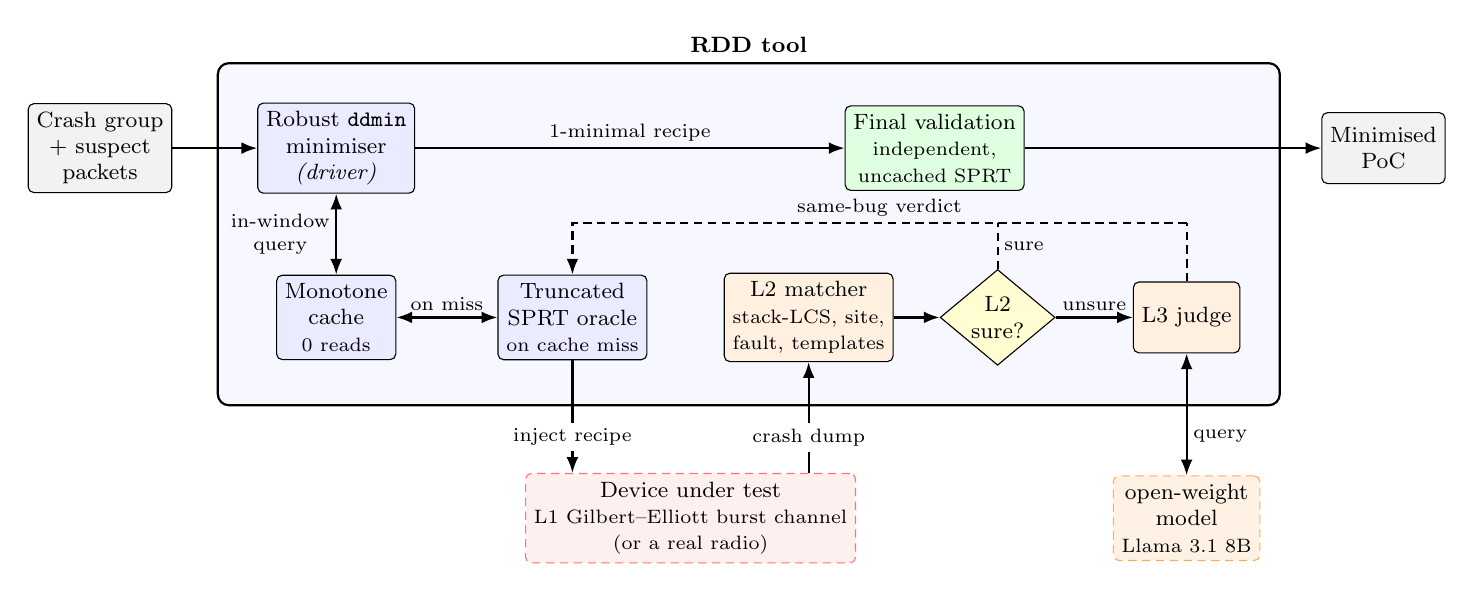
\begin{tikzpicture}[
  font=\footnotesize,
  >={Latex[length=2mm]},
  base/.style={draw,rounded corners=2pt,align=center,minimum height=9mm,inner sep=3pt},
  io/.style={base,fill=black!5},
  proc/.style={base,fill=blue!8},
  idy/.style={base,fill=orange!12},
  gate/.style={base,fill=green!12},
  ext/.style={base,fill=red!6,draw=red!55,densely dashed},
  dec/.style={draw,diamond,aspect=1.2,align=center,inner sep=1pt,fill=yellow!18},
  flow/.style={->,thick},
  fb/.style={->,thick,densely dashed},
  fbline/.style={thick,densely dashed},
  lab/.style={font=\scriptsize,inner sep=2pt,align=center},
]
% top row
\node[io]   (in)    at (0,0)       {Crash group\\$+$ suspect\\packets};
\node[proc] (ddmin) at (3.0,0)     {Robust \texttt{ddmin}\\minimiser\\\textit{(driver)}};
\node[gate] (fv)    at (10.6,0)    {Final validation\\{\scriptsize independent,}\\{\scriptsize uncached SPRT}};
\node[io]   (poc)   at (16.3,0)    {Minimised\\PoC};
% oracle + identity row
\node[proc] (cache) at (3.0,-2.15)  {Monotone\\cache\\{\scriptsize 0 reads}};
\node[proc] (sprt)  at (6.0,-2.15)  {Truncated\\SPRT oracle\\{\scriptsize on cache miss}};
\node[idy]  (l2)    at (9.0,-2.15)  {L2 matcher\\{\scriptsize stack-LCS, site,}\\{\scriptsize fault, templates}};
\node[dec]  (l2d)   at (11.4,-2.15) {L2\\sure?};
\node[idy]  (l3)    at (13.8,-2.15) {L3 judge};
% outside-the-tool resources (below the boundary)
\node[ext]  (dev)   at (7.5,-4.7)  {Device under test\\{\scriptsize L1 Gilbert--Elliott burst channel}\\{\scriptsize (or a real radio)}};
\node[ext,fill=orange!10,draw=orange!65] (model) at (13.8,-4.7) {open-weight\\model\\{\scriptsize Llama 3.1 8B}};
% ---- arrows ----
\draw[flow] (in) -- (ddmin);
\draw[flow] (ddmin) -- node[lab,above]{1-minimal recipe} (fv);
\draw[flow] (fv) -- (poc);
\draw[<->,thick] (ddmin) -- node[lab,left]{in-window\\query} (cache);
\draw[<->,thick] (cache) -- node[lab,above]{on miss} (sprt);
% the SPRT injects into the external device (call leaves the tool); the device
% returns a crash dump (re-enters); inject/dump labels carry a white fill only
% out here on the white background, to break the line they sit on
\draw[flow] (sprt) -- node[lab,fill=white,pos=0.68]{inject recipe} (dev.north -| sprt);
\draw[flow] (dev.north -| l2) -- node[lab,fill=white,pos=0.32]{crash dump} (l2);
\draw[flow] (l2) -- (l2d);
% L2's decision: unsure escalates to L3 (single arrow); sure goes to the bus
\draw[flow] (l2d) -- node[lab,above]{unsure} (l3);
\draw[<->,thick] (l3) -- node[lab,right,pos=0.68]{query} (model);
% verdict bus: the sure path from L2 and L3's answer both drop into one horizontal
% line that carries the same-bug verdict back to the SPRT (no triangle)
\coordinate (busy) at (0,-0.95);
\draw[fbline] (l2d.north) -- node[lab,right]{sure} (l2d.north |- busy);
\draw[fbline] (l3.north)  -- (l3.north |- busy);
\draw[fb] (l3.north |- busy) -- node[lab,above]{same-bug verdict} (sprt.north |- busy) -- (sprt.north);
% ---- boundary ----
\begin{scope}[on background layer]
  \node[draw,thick,rounded corners,fill=blue!3,fit=(ddmin)(fv)(cache)(sprt)(l2)(l2d)(l3),inner sep=5mm,
        label={[font=\footnotesize\bfseries]north:RDD tool}] {};
\end{scope}
\end{tikzpicture}%
}
\caption{The RDD tool and the two calls that leave it.}
\label{fig:pipeline}
\end{figure*}

\subsection{The over-the-air medium (L1)}

The medium is the lowest of the three layers Fig.~\ref{fig:pipeline} labels L1 to
L3, the other two being the tiers of the identity oracle. Both RDD and
\textsc{AirBugCatcher} are evaluated on a software target (the Zephyr controller
compiled for its host-native \texttt{unit\_testing} target, without radio
hardware), so the medium is simulated. Each attempt passes through a
\emph{Gilbert--Elliott} burst channel~\cite{gilbert1960,elliott1963} applied per attempt, a two-state
Markov chain whose ``bad'' state raises the loss rate for a few attempts, on top
of which a flakiness layer decides whether an attempt registers the crash: a
true reproducer is missed on about 0.44 of valid attempts, an attempt fails to
connect on 0.02 to 0.27 depending on the state, and a non-reproducing recipe is
reported as crashing, with the target's own dump, on 0.02 to 0.07 (a
\emph{phantom} crash). The miss rate, 0.44, is our choice, not a wireless measurement; it lies in the
upper range of the per-test failure frequencies of a flaky-test rerun
corpus~\cite{flakeflagger2021}, so that a single attempt is unreliable. The
phantom rates are ours as well. In every
reported run RDD resets the connection before each attempt, which in the
simulator resamples the channel state and makes attempts independent; the burst
structure therefore does not affect RDD's numbers, and the baseline, which reads
each candidate once, is not affected by it either.

\subsection{The truncated-SPRT reproduction oracle}

RDD decides each query with a truncated Sequential Probability Ratio Test
(SPRT)~\cite{sprt1945}. Rather than trust one attempt, it repeats the attempt and
accumulates the outcomes into a decision with a bounded error. The test weighs
$H_0$, that the recipe reproduces only at some low background rate $p_0$, against
$H_1$, that it reproduces at a high rate $p_1$; each attempt adds evidence, and
the test stops when the log-likelihood ratio crosses one of Wald's thresholds,
$\log((1-\beta)/\alpha)$ above or $\log(\beta/(1-\alpha))$ below, or when a fixed
budget of attempts is spent. $\alpha$ is the chance of wrongly accepting a
non-reproducing recipe (a false credit) and $\beta$ the chance of rejecting a
real one. The bound on $\alpha$ holds when the attempts are independent and the
non-reproducer's true rate is at most $p_0$; a true rate strictly between $p_0$
and $p_1$, the \emph{indifference zone}, is not covered by the SPRT's error bounds, a limitation intrinsic to the method that the deep-noise regime of
Section~\ref{sec:evaluation} exhibits. The prototype uses $\alpha = 0.01$,
$\beta = 0.10$, $p_0 = 0.05$, $p_1 = 0.55$ and a budget of sixteen valid attempts;
$p_0$ sits above the phantom rate an independent attempt sees on average (0.03; the
bad-state rate of 0.07 alone would exceed it) and $p_1$ near the modelled reproduce rate, so both preconditions hold in the simulator by choice of parameters. Two
departures from Wald's test bias it towards the safe answer: an inconclusive test
at the budget is ruled ``no'', so the realised miss rate can exceed $\beta$, and a
``yes'' additionally requires at least three valid attempts. Failed connections
are discarded, not counted as misses, though eight of them end a test as ``no''. Given the committed judge verdicts, every run replays exactly.

\subsection{The monotone result cache}

Within the starting window found for one bug, RDD caches decided verdicts and
answers by monotone closure: a superset of a known reproducer reproduces, a
subset of a known non-reproducer does not. Only verdicts that crossed a test
boundary are cached; a wrong decided verdict, which occurs with probability up
to $\alpha$ or $\beta$, propagates through the closure and is caught only by the
final validation. The closure is sound only if the starting window is free of
suppressors, which holds when the uncached probes that selected it were correct
and the bug has a single cause; outside the starting window the driver does not
use the cache.

\subsection{The two-tier crash-identity oracle (L2\texorpdfstring{$\rightarrow$}{ to }L3)}

An attempt that crashes must be recognised as the target bug. Under noise the same
crash arrives with a truncated backtrace, lost top frames or interleaved log
lines, so a match on the recorded trace fails. RDD uses a cost-gated cascade in the manner of
\emph{FrugalGPT}~\cite{frugalgpt2023}: a deterministic matcher first, a language
model only for what it cannot settle.

The matcher (L2) compares two reports with four signals: a longest-common-subsequence
alignment of the top five backtrace frames (weight 0.55), a Jaccard overlap of
crash-site tokens (0.25), a coarse fault-class check (0.05), and an overlap of log
templates mined online with \emph{Drain}~\cite{drain2017} (0.15), which ignores
the volatile details. The threshold was fixed at 0.5 before any calibration. A
post-hoc sweep on the six real bugs, over 360 same-bug and 360 different-bug pairs
produced by the report-variation model with no held-out set, gives an area under
the ROC curve of 0.993, a Youden~\cite{youden1950} optimum of 0.529 and balanced
accuracy on a plateau over $[0.45, 0.80]$; it supports the choice but does not
show that it generalises. % l2_threshold_eval.json

The judge (L3) is consulted only when the matcher says ``different'' with a score
in $[0.05, 0.5)$, a band that holds about half of the different-bug pairs in the
calibration set. It is a single open-weight model (Llama~3.1~8B~\cite{llama3_2024})
asked whether the two reports describe the same bug; it sees the same reports the
matcher saw. It is served locally through Ollama as the library tag
\texttt{llama3.1:8b}, a 4-bit build, at temperature 0 with a fixed seed and
JSON-constrained output. On an offline set of escalated pairs it recovered every same-bug pair the
matcher had abstained on (57 of 57) and also accepted every different-bug pair
(40 of 40); in the benchmark runs' caches it answered ``same'' every time. % l3_judge_eval.json
The cascade therefore rejects a different-bug report only when the matcher scores
it below 0.05; cross-bug discrimination rests on the matcher, and the judge is a
recall aid. No experiment in this report presents a different bug's report to the
in-loop oracle, so the consequence, crediting a recipe that reproduces a different
bug, is not measured; Section~\ref{sec:evaluation} lists the experiment that
would.

Report variation itself is a model. Each observed crash is emitted from the
captured base dump with the backtrace truncated with probability 0.35, its top
frames lost with 0.20, a frame added or removed with 0.15, an unrelated log line
interleaved with 0.40 and the report severely garbled with 0.08; the rates are
ours, chosen as a moderate operating point. The identity layer's advantage over
exact matching in Section~\ref{sec:evaluation} is a function of these rates.

\subsection{Non-monotone-robust delta debugging}

Delta debugging~\cite{ddmin2002} assumes monotonicity: if a set of packets crashes
the device, adding packets does not stop the crash. A \emph{suppressor}
packet in the window violates it, and if the full window contains one, the first
test fails and \texttt{ddmin} returns nothing. RDD's driver first tests the full
window with the uncached oracle; if it does not crash, it searches for a crashing
starting window by bounded leave-$k$-out and build-up probing, cheapest first,
and only then runs \texttt{ddmin} inside that window, where the cache is sound.
When the full window did not crash, each excluded packet is then added back once: if adding it makes the crash
disappear, it is reported as a suppressor. Strictly pairwise suppressors are out of
scope. The result is 1-minimal with respect to the oracle's verdicts: a false
``no'' on a single-packet removal leaves an unnecessary packet, which the size-gap
metric of Section~\ref{sec:evaluation} measures.

\subsection{The final validation}

RDD credits a recipe only after a second, uncached sequential test with a tighter $\beta$ (0.01) on the same noisy channel. For a given non-reproducing recipe both the
in-loop verdict and this re-confirmation must wrongly accept it, each with
probability at most $\alpha$ when the two runs are independent and the recipe's
true rate is at most $p_0$; over a reduction that queries $k$ non-reproducing
candidates the per-campaign bound is about $k\alpha^2$. Identity errors are shared
by both runs and are not covered by the bound. Genuine and false credit are
assigned by the evaluation, not by the tool: the scorer compares each credited
recipe to a channel-off run of the device.

\subsection{Positioning: a SWOT view}

\textbf{Strengths.} Delta debugging returns with its 1-minimality relative to the
oracle, where \textsc{AirBugCatcher} enumerates up to a fixed size. The false-credit
rate is $\alpha$-bounded under stated preconditions, and the re-confirmation
squares it. The identity cascade escalates only the uncertain residual, so the
model is cheap and its verdicts can be committed and replayed.

\textbf{Weaknesses.} The evaluation is a simulator whose two noise models,
phantom crashes and report variation, produce the advantage
(Section~\ref{sec:evaluation}); RDD costs 3.5 to 5 times the baseline's device reads on the two
benchmarks and six to ten times on the suppressor bug; the judge does not discriminate on the pairs it receives; the
indifference zone leaves the deepest noise unrecoverable; the matcher's threshold
is calibrated on six bugs with no held-out set.

\textbf{Opportunities.} Measuring the phantom and variation rates on a real link
turns the sensitivity table into a prediction; cross-target campaigns on other
stacks with tools such as \textsc{U-Fuzz}~\cite{ufuzz2024} would calibrate the
identity layer on held-out bugs; a calibrated panel could replace the single judge.

\textbf{Threats.} The method assumes a device that can be reset between attempts;
real radios show correlated behaviour the reset may not remove; a single model
judge carries a systematic bias. These shape the experiments proposed in
Section~\ref{sec:evaluation}.

\section{Evaluation}\label{sec:evaluation}

We tested the approach with a working prototype and treat the results as
proof-of-concept evidence for a research direction, not as a field result. The
comparison is against a re-implementation of \textsc{AirBugCatcher}'s reproduction
strategy~\cite{airbugcatcher2024}: bounded enumeration of suspect-packet
combinations up to three packets, in order of proximity to the crash, one
attempt per candidate, accepting the first candidate whose crash carries the
expected signature. It is our reading of the published method, not the authors'
tool, and it runs with no trial-time budget, so it enumerates more candidates
than the original would. Both tools face the same simulated device and channel,
so a difference between them is a difference between the two strategies
\emph{under our noise model}; Section~\ref{ssec:eval-noise} measures how much of
the difference the model itself contributes.

Every arm is scored by the same rule. A campaign is a \emph{genuine} reproduction
if the arm credited a recipe \emph{and} that recipe crashes the target with the
channel switched off, a ground truth the tools never see; it is a \emph{false
credit} if the arm credited a recipe that does not. A recipe the tool returns but
declines to validate counts for neither. The \emph{size gap} is the mean number of
packets a genuine recipe carries beyond the true minimum, and \emph{reads} counts
device attempts per campaign. A third arm, the baseline with one confirming
re-run before it credits a candidate, is the confirmation control; its reads are in
Table~\ref{tab:headlines}.
Table~\ref{tab:headlines} summarises the results.

\begin{table*}[!t]
\renewcommand{\arraystretch}{1.3}
\caption{Main results on the same simulated channel. Size gap is the mean extra
packets over the true minimum, over genuine reproductions only; the best value of
each scored column within a benchmark is in bold. RDD's synthetic false credit is one
campaign in 75,000, which rounds to 0.000.}
\label{tab:headlines}
\centering
\begin{tabular*}{\textwidth}{@{\extracolsep{\fill}}l l c c c c@{}}
\toprule
Benchmark & Configuration & Genuine $\uparrow$ & False credit $\downarrow$ & Size gap $\downarrow$ & Reads\\
\midrule
Real head-to-head            & \textsc{AirBugCatcher}                & 0.759 & 0.137 & 0.483 & 9\\
{\footnotesize 6 bugs, 336 campaigns} & \textsc{AirBugCatcher} $+$ 1 confirmation & 0.708 & 0.006 & 0.931 & 24\\
                             & RDD                                   & \textbf{0.848} & \textbf{0.000} & \textbf{0.117} & 45\\
\addlinespace
Resilience at scale          & \textsc{AirBugCatcher}                & 0.266 & 0.632 & 0.518 & 41\\
{\footnotesize 15,000 bugs, 75,000 campaigns} & \textsc{AirBugCatcher} $+$ 1 confirmation & 0.359 & 0.090 & 0.922 & 342\\
                             & RDD                                   & \textbf{0.824} & \textbf{0.000} & \textbf{0.206} & 143\\
\bottomrule
\end{tabular*}
\end{table*}

\subsection{Real bugs, head to head}

The evaluation uses six controller bugs, labelled A--F, in the Zephyr Bluetooth
Low Energy stack compiled for Zephyr's host-native \texttt{unit\_testing} target.
One is a disclosed vulnerability with a CVE identifier, a division by zero in
connection-parameter handling; the other five are reachable controller faults
exercised through harness patches on the same vulnerable controller, one of them
sharing the first bug's binary. Each bug has a fixed window of eight (A, B) or
five (C--F) packets whose minimal recipe has one or two packets, so the
enumeration baseline reaches every true minimum within its first six candidates
when the channel lets it; the difficulty of these bugs lies in the noise, not in
the search. The committed crash dump of bug B carries no backtrace, which makes
exact matching stronger on B than elsewhere.

Through the full pipeline (a synthesised fuzz trace, a crash-grouping front end given to both tools, which is
our deterministic matcher, then each bug's fixed window and either minimiser), RDD
recovers 0.848 of reproductions with no false credit in 336 campaigns; the
baseline recovers 0.759 with 0.137 false credit. % headtohead.json
Over the eight runs RDD spans $[0.76, 0.90]$ and the baseline $[0.67, 0.81]$,
paired per run. RDD's recipes are also tighter: 0.12 extra packets against 0.48,
and 0.89 of them exactly minimal. Both tools suffer the shared front end, which
sometimes assigns a trace to the wrong bug; on correctly grouped traces the rates
are 0.920 and 0.824. Reduced directly from each bug's window on the truth-table
oracle over thirty runs, RDD recovers 0.933 against the baseline's 0.867
(false credit 0.089). % anchor.json
The cost is reads: about 45 device attempts per campaign against 9, spent on the
sequential test's repeated trials; escalations to the language model are identity
checks on attempts already made, not extra reads.

The baseline's false credit is a consequence of accept-first: it books the first
candidate whose crash carries the expected signature, and under our channel a
non-reproducing candidate occasionally does. One confirming re-run removes almost
all of it (0.137 to 0.006) at 24 reads, but costs recall (0.708) because a true
reproduction must now survive both the channel and exact matching twice. RDD produced no false credit in these 336 campaigns, in the 180 truth-table campaigns
on A--F or in the 30 on the suppressor (95\,\% upper bounds on its rate 0.9\,\%,
1.7\,\% and 10\,\%), and one in the 75,000 synthetic campaigns of
Section~\ref{ssec:eval-scale} (a rate of $1.3\times10^{-5}$; upper bound 0.006\,\%). The tool's property is the
$\alpha$-bounded rate of Section~\ref{sec:our_approach}; zero is the measured outcome.

On the real suppressor bug, where a later packet hides the crash (its harness prints
no backtrace, so the target emits bug A's dump), the baseline
recovers 0.875 with 0.125 false credit; RDD recovers every one of the eight
head-to-head campaigns, and 0.9 of the thirty truth-table runs, with no false credit
in either;
bare delta debugging, started from the non-crashing full window, returns nothing,
which is the cost RDD's own choice of \texttt{ddmin} would incur without its
starting-window search (Section~\ref{ssec:eval-levers}).

\subsection{How much is the noise model}\label{ssec:eval-noise}

Two assumed models drive the comparison: the channel's phantom crashes (a
non-reproducing recipe reported as crashing with the target's own dump, 0.02 to
0.07 per attempt), and the crash-report variation applied to every observed crash
(Section~\ref{sec:our_approach}). Table~\ref{tab:noise} repeats the thirty-run
truth-table experiment with each switched off.

\begin{table}[!t]
\renewcommand{\arraystretch}{1.2}
\caption{The six real bugs, thirty runs each, under weaker noise models. Cells are
genuine / false credit over 180 campaigns, so a rate carries a standard error of
about 0.02; reads for the last row are given in the text.}
\label{tab:noise}
\centering
\footnotesize
\setlength{\tabcolsep}{3pt}%
\begin{tabular}{@{}lccc@{}}
\toprule
Noise model & Baseline & $+$ 1 confirmation & RDD\\
\midrule
as committed            & 0.867 / 0.089 & 0.761 / 0.006 & 0.933 / 0.000\\
report variation off    & 0.911 / 0.067 & 0.911 / 0.000 & 0.928 / 0.000\\
phantom crashes off     & 0.933 / 0.000 & 0.750 / 0.000 & 0.933 / 0.000\\
both off                & 0.978 / 0.000 & 0.933 / 0.000 & 0.928 / 0.000\\
\bottomrule
\end{tabular}
\end{table}

The baseline's false credit vanishes exactly when phantom crashes do, and its
recall gap closes when report variation does; with both off it recovers 0.978
with no false credit at about ten reads per campaign, ahead of RDD's 0.928 at
about 47. RDD's results are almost invariant to the two models because the
sequential test absorbs the phantoms and the identity layer absorbs the
variation, which is what they were built for. The comparison is therefore a
statement about the noise the medium is assumed to produce: where a device
reports spurious crashes of the target signature or garbles its reports, RDD
recovers more at higher cost; where it does neither, plain enumeration is the better tool, and a confirming re-run
buys the same recall as RDD at about a third of its reads.

\subsection{Resilience at scale}\label{ssec:eval-scale}

Because only a handful of real emulable bugs exist, we probe robustness with a
synthetic corpus anchored to the real target: fifteen thousand bugs across six
regimes (standard, high-cardinality, suppressor, far-trigger, deep-noise, and
wide-window), 75,000 campaigns per tool. The regimes were chosen by us to stress
structures known to trouble the two search strategies: large input spaces,
non-monotone suppressors, awkward trigger positions, and noise deep enough to push
a true reproduce rate into the SPRT's indifference zone; only the last stresses
RDD. About a third of the population (0.79 in high-cardinality, 0.24 to 0.27
elsewhere) has minimal recipes larger than the baseline's three-packet cap and is
unreachable for it by construction. At this scale the identity layer's second tier
is a rule that accepts a report containing the target's crash-site symbol or
file; it uses the target's known site, so it stands in for the judge's recall
rather than bounding it, and the sweep runs with no model.

RDD averages 0.824 genuine recovery with one false credit in 75,000 campaigns, a
five-packet sub-recipe of a six-packet minimum in the suppressor regime; the baseline averages
0.266 with 0.632, and with one confirming re-run 0.359 with 0.090 at 342 reads
per campaign, because confirmation removes the phantom stop that ended its
campaigns early (Fig.~\ref{fig:regimes}). % resilience.json OVERALL
Each campaign draws its own noise stream, and the bootstrap intervals resample bugs,
not campaigns, since a bug's five campaigns are correlated: RDD $[0.820, 0.829]$, baseline $[0.261, 0.272]$. They quantify
sampling error over our generator, not agreement with real bugs. RDD's reads are
roughly 143 per campaign against the baseline's 41.

\begin{figure}[!t]
\centering
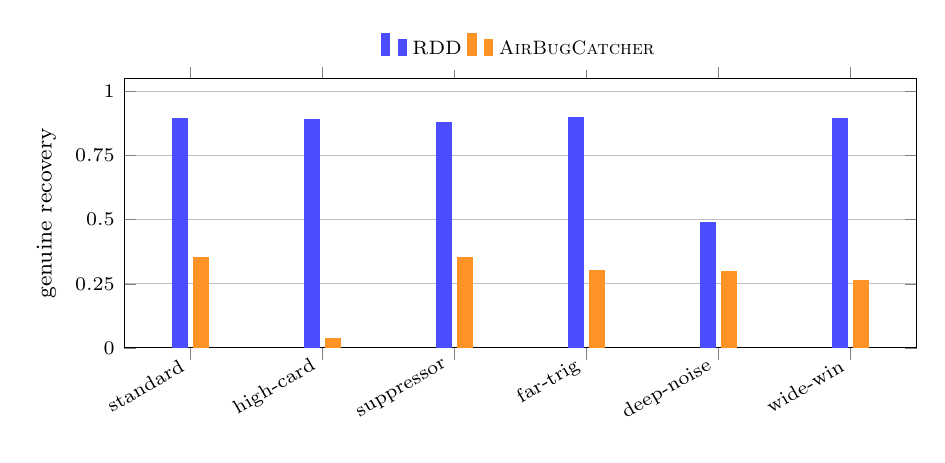
\begin{tikzpicture}
\begin{axis}[
  width=0.96\columnwidth, height=5.0cm,
  ybar, bar width=5.5pt,
  ymin=0, ymax=1.05,
  ylabel={genuine recovery},
  ylabel style={font=\footnotesize},
  symbolic x coords={standard,high-card,suppressor,far-trig,deep-noise,wide-win},
  xtick=data,
  x tick label style={rotate=30,anchor=east,font=\scriptsize},
  ytick={0,0.25,0.5,0.75,1.0},
  yticklabel style={font=\scriptsize},
  legend style={at={(0.5,1.03)},anchor=south,legend columns=2,font=\scriptsize,draw=none},
  enlarge x limits=0.1,
  ymajorgrids,
]
\addplot+[fill=blue!70,draw=blue!70] coordinates {(standard,0.896)(high-card,0.891)(suppressor,0.879)(far-trig,0.897)(deep-noise,0.490)(wide-win,0.893)};
\addplot+[fill=orange!85,draw=orange!85] coordinates {(standard,0.351)(high-card,0.037)(suppressor,0.352)(far-trig,0.300)(deep-noise,0.296)(wide-win,0.261)};
\legend{RDD, \textsc{AirBugCatcher}}
\end{axis}
\end{tikzpicture}
\caption{Genuine recovery per regime (12,500 campaigns each). RDD stays above 0.87
except in deep-noise (0.49, the SPRT indifference zone); the baseline is worst on
high-cardinality inputs, most of which exceed its cap.}% resilience.json per-regime point estimates
\label{fig:regimes}
\end{figure}

The regimes separate the mechanisms. The baseline does best in the standard and
suppressor regimes (0.351, 0.352) and fails almost completely on high-cardinality
inputs (0.037). RDD stays between 0.88 and 0.90 everywhere except deep-noise, where
it drops to 0.490: at that severity the per-attempt reproduce rate of a true
recipe falls to 0.23--0.45 for four fifths of the bugs (0.36 at the modal severity),
inside the indifference zone $(p_0, p_1) =
(0.05, 0.55)$, so the truncated test mostly ends inconclusive, which the tool
scores as a non-reproduction rather than a credit. Its recipes there are no
tighter than the baseline's (0.66 against 0.65 extra packets). Narrowing the band
or raising the trial budget reduces the zone at the price of more reads; RDD
accepts the lost recall to keep the false-credit bound, which is the purpose of
the gate.

\subsection{Where the advantage comes from}\label{ssec:eval-levers}

RDD has several components, and Table~\ref{tab:levers} adds them one at a time
on the real bugs, reducing each bug directly from its window without the shared
front end of Table~\ref{tab:headlines}. These are 48 campaigns (six bugs, eight
runs), so the baseline's recall is 0.771 here (live binary, eight runs) against 0.759 through
the front end and 0.867 on the truth table; its per-run range is $[0.67, 1.00]$.

\begin{table}[!t]
\renewcommand{\arraystretch}{1.2}
\caption{Each component's contribution on the real bugs; each row adds one. The
oracle removes false credit, the identity layer restores recall, the minimiser
survives the suppressor.}
\label{tab:levers}
\centering
\setlength{\tabcolsep}{4pt}%
\begin{tabular}{@{}lccc@{}}
\toprule
 & Genuine & False credit & Genuine\\
Configuration & (A--F) & (A--F) & (suppressor)\\
\midrule
\textsc{AirBugCatcher} baseline    & 0.771 & 0.188 & 0.875\\
$+$ SPRT oracle                    & 0.688 & \textbf{0.000} & 0.000\\
$+$ two-tier identity              & \textbf{0.917} & 0.000 & 0.000\\
$+$ robust minimiser (full RDD)    & 0.917 & 0.000 & \textbf{1.000}\\
\bottomrule
\end{tabular}
\end{table}

Replacing accept-first enumeration by the sequential oracle and \texttt{ddmin}
brings false credit from 0.188 to zero, and it stays there as the other
components are added. % levers.json oracle_fc_invariance
This step changes two things at once, the oracle and the search, so we attribute
to it only the false-credit result; its effect on recall (0.771 to 0.688, per-run
range $[0.33, 1.00]$) is within run-to-run variation. On the suppressor bug it
scores zero, because \texttt{ddmin} bails on a masked full window. Replacing the
exact matcher by the two-tier identity raises recall from 0.688 to 0.917
(+0.229), the largest single gain, and it is a gain against the modelled report
variation of Section~\ref{ssec:eval-noise}. The robust minimiser changes nothing
on the monotone bugs and takes the suppressor from zero to every campaign, by
finding a suppressor-free starting window where plain \texttt{ddmin} finds none.

\subsection{Threats to validity}

\textbf{The simulator.} The device is a deterministic host build of the Zephyr
controller; the channel is a Gilbert--Elliott burst process whose miss rate,
0.44, is our choice rather than a wireless measurement (it lies in the upper
range of the per-test failure frequencies of a flaky-test rerun
corpus~\cite{flakeflagger2021}) and whose phantom rates are ours; the
crash-report variation is a model with rates we chose (backtrace
truncation 0.35, top-frame loss 0.20, frame churn 0.15, log interleaving 0.40,
severe garbling 0.08). Section~\ref{ssec:eval-noise} shows that the headline
advantage is a consequence of these models. A phantom crash is modelled as
carrying the target's own signature, the case that defeats exact matching; a
device that phantoms other crashes, or none, would favour the baseline. RDD
resets the session before every attempt, which in the simulator makes attempts
independent; the burst structure therefore never affects RDD, and the effect of
correlated attempts, which violate the sequential test's precondition, is not
evaluated.

\textbf{The baseline.} It is our re-implementation of one published strategy at
a fifth to a quarter of RDD's reads. The confirmation control shows that one confirming
re-run removes almost all of its false credit; a budget-matched variant with a
different search was not run.

\textbf{Identity.} The deterministic matcher was calibrated post hoc on the same
six bugs (360 same-bug and 360 different-bug pairs generated by the variation
model, no held-out set). The judge accepted every one of the 40 different-bug
pairs the cascade escalates to it and every one of the 57 same-bug pairs, so the
cascade rejects a different-bug report only when the matcher scores it below the
escalation floor, which covers about half of the different-bug pairs in the
calibration set. No experiment here presents a different bug's report to the
in-loop oracle, because each harness emits only its target's crash; the resulting
risk, crediting a recipe that reproduces a different bug, is unmeasured. The
judge's verdicts are replayed from a committed cache; live inference is not
guaranteed bit-reproducible, although re-judging all 386 cached pairs with the
same model tag (Ollama 0.34.2, 24 September 2026) returned every verdict
unchanged.

\textbf{Construct.} ``Genuine'' is defined against a channel-off run of a
deterministic binary. A bug that appears only with channel noise is scored as a
non-reproduction, a bias that trades recall for the false-credit bound; the
truncated test's forced ``no'' is the mechanism we expect behind most of RDD's
deep-noise loss. The code carries an
optional identity guard for binaries that ship several bugs; it is off in every
reported run. Six bugs, one stack, one CVE and one synthetic fault mechanism bound
what the numbers can say.

\subsection{Proposed experiments}

The results order the research plan. First, measure the two assumed rates on a
real link: replay recovered recipes over a software-defined radio and record how
often a non-reproducing recipe crashes the device, with which signature, and how
often the same crash is reported differently; the noise-sensitivity table then
becomes a prediction. Second, present different-bug reports to the in-loop oracle,
on a binary that ships several reachable bugs in one window, and measure
cross-bug credit. Third, run correlated attempts, with reset and settling
disabled, to find the burst regime at which the sequential test's error bound
fails. Fourth, repeat the study on other Bluetooth, Wi-Fi and cellular stacks
using public fuzzing logs, with the matcher's threshold calibrated on held-out
bugs. Fifth, replace the single judge by a calibrated panel evaluated against
human agreement (Cohen's $\kappa$~\cite{cohenkappa1960}), since a judge that never
rejects adds recall but no discrimination. The indifference zone remains; an
adaptive trial budget that spends reads only in the noisiest cases is the
mitigation to test.

\section{Related work}\label{sec:related_work}

RDD integrates several established fields: input minimisation, over-the-air
fuzzing, oracle stabilisation, language models for testing, crash deduplication,
and commercial tools. While each area is well developed individually, we know of no
prior work combining them through adaptive minimisation guided by a statistical
reproduction oracle on a noisy wireless stack.

\subsection{Input minimisation under noisy verdicts}

The primary algorithm, \texttt{ddmin}~\cite{ddmin2002}, is a general-purpose
reducer that identifies a locally minimal failing input. It has been the standard
minimiser in compiler testing and bug reproduction for approximately twenty years;
\textsc{C-Reduce}~\cite{creduce2012} and \textsc{Perses}~\cite{perses2018} are
prominent syntax-guided refinements for structured source programs.
Hierarchical Delta Debugging~\cite{hdd2006} adapts \texttt{ddmin} for
tree-structured inputs, which differs from the noisy verdict problem addressed
here. Probabilistic Delta Debugging (\textsc{ProbDD})~\cite{probdd2021} employs a
Bayesian estimate to determine which elements are significant and to reduce oracle
calls. However, these methods treat the oracle as \emph{deterministic}, making
assumptions about the input rather than the verdict. Probabilistic Monotonicity
Assessment (\textsc{PMA})~\cite{pma2025} departs from this,
modelling the search space's \emph{monotonicity} probabilistically to avoid
redundant tests. \textsc{PMA} is the closest related work; it cites noise and
intermittent failures as motivation, but it accepts each verdict as given and does
not \emph{stabilise} it with repeated trials, sequential tests or an error bound. All these methods assume a
reliable oracle, which wireless environments do not provide, so \texttt{ddmin}'s
1-minimality guarantee does not hold. RDD adopts a different strategy: it maintains
a classical search but prioritises producing a reliable verdict, complementing
rather than competing with these minimisers. Delta debugging has previously been
applied to non-deterministic targets. For example, Pontolillo and
Mousavi~\cite{quantumdd2024} reduce quantum-program regressions using a
fixed-sample property check on a simulator, not a sequential, bounded-error
decision on a real channel.

\subsection{Wireless fuzzing: discovery versus reproduction}

Over-the-air protocol fuzzing is a well-established field.
\textsc{SweynTooth}~\cite{sweyntooth2020} identified eleven BLE vulnerabilities
in chips from seven vendors, and \textsc{BrakTooth}~\cite{braktooth2022} eighteen in
Bluetooth Classic devices from eleven vendors. Both projects conclude at discovery, requiring analysts to
manually construct a clean PoC. \textsc{U-Fuzz}~\cite{ufuzz2024} advances further:
after stateful fuzzing of IoT and 5G protocols, it performs a post-fuzzing step to
identify the minimal set of mutated packets that cause a crash. This makes U-Fuzz
RDD's closest counterpart, but the distinction lies in the oracle. U-Fuzz walks
backwards from the crash replaying one mutated packet at a time in a fresh session
until the crash recurs, states no retry policy, and labels crashes whose
reproduction is unstable as anomalies, while RDD employs a sequential,
bounded-error verdict.
\textsc{AirBugCatcher}~\cite{airbugcatcher2024} is the most direct comparator, as it
also addresses noisy-verdict problems. However, it examines suspect combinations up
to a small fixed size and runs each generated test case once within a trial budget,
rather than stabilising the verdict. In its study, a plain replay baseline,
repeated five times to average out the medium, reproduced only 13 to 23 of 190
crashes on its Bluetooth target and none on the other four~\cite{airbugcatcher2024}. % AirBugCatcher RQ5, Table 7
RDD builds upon these concepts rather than competing with them. Three improvements
have been noted: bounded enumeration is replaced by \texttt{ddmin}, and one attempt
per candidate is replaced by a statistical oracle. The third improvement is in the
identity layer: \textsc{AirBugCatcher} matches crashes by exact source-line trace,
by an address-offset pattern on memory traces, or by packet state when no log
exists, and counts a crash with a non-matching identifier as ``unexpected'';
RDD uses a two-tier cascade tolerant of truncated and garbled reports.

\subsection{Oracle stabilisation and flaky tests}

The oracle problem --- determining whether an outcome is truly a failure --- has
been a focus of testing research for over a decade. Barr et
al.~\cite{oracleproblem2015} review scenarios where no perfect oracle exists, and
Luo et al.~\cite{flakytests2014} discuss flaky tests where verdicts vary across
identical runs. Both works identify the issue but do not provide a decision rule
for noisy \emph{physical} targets. The Sequential Probability Ratio Test
(SPRT)~\cite{sprt1945} addresses this by offering a rule that makes decisions within
a set budget while controlling both error rates. Applying SPRT to the reproduction
oracle introduces Wald's guarantees, reducing false credit from the baseline's
0.632 to 0.000 in all stress tests. Using a statistical test as an oracle is not new: Guderlei and
Mayer~\cite{statoracle2007} test random-output programs by comparing independent
output samples under a metamorphic relation with a fixed-sample hypothesis test, an
offline batch decision, whereas RDD makes sequential, bounded-error verdicts during
the reduction process.

\subsection{Language models (LLMs) as testing oracles}

Language models are now applied in testing in various ways.
\textsc{LPR}~\cite{lpr2024} combines a syntax-guided reducer with LLM-proposed
rewrites, but the model only suggests changes and the oracle remains a
deterministic recompile. \textsc{ChatAFL}~\cite{chatafl2024} allows an LLM to guide
greybox fuzzing of RFC protocols on wired targets, and
\textsc{Candor}~\cite{candor2025} uses multiple models to reach consensus and
generate oracles offline. The most structurally similar approach is
\textsc{DDOR}~\cite{ddor2026}, a recent preprint, which incorporates LLM judging
within a delta-debugging loop for chatbot over-refusal. While similar to RDD, DDOR
targets a replayable software endpoint, without wireless noise or a statistical
reproduction oracle. Another recent effort applies delta debugging to
LLM-integrated systems~\cite{ddllm2026} with semantic markers; it treats the model
as a probabilistic oracle and classifies each subset by a fixed number of repeated
trials with a failure threshold, a majority vote rather than a sequential,
error-bounded test. Ensemble frameworks differ:
self-consistency~\cite{selfconsistency2023} uses a single model's majority vote,
cross-model voting yields only minor gains once voters are
correlated~\cite{condorcetllm2024}, LLM-as-a-judge approaches approximate human
grading~\cite{llmjudge2023}, and unanimous open-weight juries review LLM-written
code offline~\cite{llmjuries2026}. RDD is fundamentally different: its L3 is a
\emph{single} crash-identity judge, used only when the deterministic L2 is uncertain,
similar to FrugalGPT-style escalation~\cite{frugalgpt2023}. The stabiliser is the
SPRT oracle, not an ensemble, and the model is used to infer identity rather than
reproduction.

\subsection{Crash identity and deduplication}

An identity layer is required to match crashes across noisy trials. Beyond exact
stack-hash matching, \emph{Drain}~\cite{drain2017} groups similar logs by mining log
templates online, and Semantic Crash Bucketing~\cite{scb2018} groups crashes based
on whether a simple program change resolves them. Igor~\cite{igor2021} clusters by
root cause using minimised execution traces, offering greater precision, but like
the others, this is an offline triage step. RDD integrates these concepts into a
two-tier identity system: a deterministic L2 that considers stack, site, fault
class, and log templates, and refers only the remaining uncertain cases to an
open-weight model~\cite{llama3_2024}. This cost-gated cascade is incorporated into
the reproduction oracle, unlike previous approaches that treat identity as a
separate triage step. The closest comparison is GPTrace~\cite{gptrace2026}, which
deduplicates crashes using language-model embeddings offline, whereas RDD's judge
determines identity during the process as part of the reproduction verdict.

\subsection{The marketplace}

Commercial wireless fuzzing is well established. Defensics~\cite{defensics} provides
Bluetooth and Wi-Fi suites that transmit malformed traffic over the air, and
Keysight's IoT Security Assessment offers similar capabilities for radio stacks
and incorporated the \textsc{BrakTooth} findings, whose research Keysight
funded~\cite{keysightiot,keysightbraktooth2021,braktooth2022}. Both tools
identify failures but do not perform minimisation. Crash triage is also commercial:
Google's ClusterFuzz~\cite{clusterfuzz} deduplicates and minimises test cases, but
only on locally executed software where results are repeatable. A market review
found no tool that combines adaptive minimisation with a non-deterministic
over-the-air target; these features are offered separately.

\subsection{Where RDD sits}

Input minimisation, wireless discovery, and crash identity are all well-developed
fields, but have not previously been combined. To our knowledge, no prior tool uses
\texttt{ddmin} with a \emph{statistical} reproduction oracle that is SPRT-stabilised
and false-credit-bounded on a non-deterministic wireless target, together with a
tiered identity cascade for the varied dumps caused by noise. Other tools are
similar but not equivalent. \textsc{U-Fuzz} minimises wireless crashes, but only
with a single replay rather than a stabilised verdict. \textsc{PMA} measures
monotonicity but does not provide a bounded-error verdict. \textsc{DDOR} reduces against a replayable
endpoint, and the LLM-system reducer votes over a fixed number of trials. The quantum reducer uses a
fixed-sample check. That is the position RDD takes.

\section{Conclusions}\label{sec:conclusions}

This report addresses a structural limitation in reproducing wireless IoT bugs.
Channel noise and device variability render the oracle non-deterministic, and once
either factor enters the test loop, exact minimisation algorithms that rely on a
stable verdict~\cite{ddmin2002} can no longer converge on the correct minimal
recipe. We propose that the software-only layer restores the stable-verdict
assumption, enabling traditional delta debugging at desktop cost with an
$\alpha$-bounded restriction on false credit. The method achieves 0.863 recovery at
zero false credit, the baseline 0.759 at 0.137, and it holds this lead under stress.
The zero-false-credit result comes chiefly from the sequential test withholding
credit from non-genuine reproductions.

Two limitations of the proof-of-concept stem from the test's design, not the method.
First, the indifference zone leaves the deepest noise undecidable~\cite{sprt1945}.
Second, the oracle's effect on \emph{genuine} recovery is intertwined with the
transition to \texttt{ddmin}, so it is claimed only for false credit, not a clear
recovery gain. The proposed experiments aim at a field-deployable wireless
reproduction oracle: real radios for the channel, new protocol stacks and fault
types, and a panel in place of the single judge. Ultimately, stabilising the verdict
lets established methods handle the remainder.



% Bibliography is driven by real \cite{} calls in the section files.
\bibliographystyle{IEEEtranS}
\bibliography{references}


% that's all folks
\end{document}
